\chapter{Requirements Elicitation}\label{chap:chap4}

\section*{}

This chapter will present in detail the first stage on the development process of this thesis, covering the initial usability requirements elicitation.

The following sections provide an analysis of the previously existing work on the project and conclusions drawn from that work, as well as the process that lead to a first redesign, based on those conclusions.

In the last section, the referred redesign, consisting in several alternative solutions, will act as a discussion material in a focus group performed with potential users of the application, in order to elicit usability requirements. All the process of the focus group, as well as all the data gathered from it, is detailed there.

\section{Previous work}

As said before, the initial work on this project encompassed the initial implementation of the concept referred on \cite{kn: Nun}, including a first prototype of an \emph{Android} mobile application. This prototype was made using \emph{Android} API level 8, being compatible with mobile devices running at least version 2.2 of the operative system.

This prototype had the following set of features \cite{kn:Gonc}

\begin{itemize}
\item Login
\item Register Account
\item Check-in
\item Check-out
\item See News Feed
\item Check
\item Submit a Comment
\item Rate a Comment from Other User
\item Plan a Journey
\end{itemize}

A more detailed explanation of those features, introducing some of the interaction flow of the prototype, is the following:

\begin{enumerate}
\item User launched the application, being prompted to login or to register a new account if he had not created one yet. If the user does not have an account, he has to register and then he is guided to the login screen.

\item User had the possibility to check-in on a vehicle by two methods: manual insertion of the public transport stop names (origin and destination), or by GPS, where the user location was used in order to fetch the nearest stops, marking a chosen one as the origin, and choosing the destination from one of the given possibilities, thus marking the journey is making at that given moment.

\item While checked-in (\emph{and only then}) the user could perform actions like submit a new comment for the selected journey (that could be written text comment, to a maximum of 150 characters, or a predefined categorised comment, rating aspects of the vehicle, which was converted to text afterwards), check a news feed with comments from other users made for the same journey, and rate the correctness of comments from other users.

\item User could also perform check-out, in order to mark the end of the journey.

\item User could check his/her profile in order to check their number of points (awarded from submitted comments) and change settings like his nickname or if that nickname will be hidden from other users (in their news feed).

\item Finally, users could plan a journey for the future, setting the origin and destination stops, and choosing a date and time. Ten minutes before the planned journey, the user receives a notification asking if he wants to receive information for that journey (thus checking-in on the journey).
 
\end{enumerate}

The developed prototype was the subject of a test in the field, performed in London with real bus users. A certain number of tasks, exploring all the features above mentioned, were given to the users, in order to measure the average execution time of each task.

Despite the obtained results (average times for task completion were considered positive), there were tasks that could or should have better accomplishment times, given their importance in the whole user experience and utility.
For instance, planning a journey takes more than 80 seconds, on average (despite being referred that happens due to a bug in a auto-complete feature), but there are a lot more features taking more than 30 seconds on average to be accomplished (check-in in, whether through the manual method or using GPS location, and rating a comment from other user). 

Regarding the check-in functionalities, this can be a problem since it is a feature used on a critical part of the application - check-in is required to access several other main use cases. Making this process too extensive or making those features only accessible to checked-in users may lead to loss of interest by potential users.

One of the possible causes to this unwanted results is the fact that the check-in options are not accessible at a user's view level after logging in with his account - in order to perform check-in, users had to press the \emph{Android} Menu button (which prompts up the context menu to the user, where they would find those options).

The same principle is valid for the check-out feature, as the button who triggers it is also found in the context menu. 

Despite the results obtained for this task were much better, that is probably due to the fact that, in order to perform check-out, an user has to check-in in the first place, learning the place where the check-out button is when he's faced with the check-in task.

Still, no visual element whatsoever gives the user the information that the context menu is available to be shown. We should not rely on previous experience that the final user may have with the platform/operative system for which we are designing an interface, specially if that possible experience includes gestures, buttons or other interaction triggers that may be unfamiliar for the user in similar contexts or not visible.

There was another task with average accomplishment time exceeding 30 seconds - submitting a written comment - though it's fair to assume that most of that time consists in writing the desired comment, and it is not necessarily tied to a disadvantage of the interface.

Another measurement taken was a quantitative value (from one to five) representing the appraisal of a given task, concerning its difficulty, so that one represents a very difficult task to execute, and five represents an easy task.
Here, the tasks that could have had better results were related to the notification system (informing a user that he has a planned journey soon, asking if he wants to receive information from it and check-in), as well as rating other users comments. 

This last concept was perceived as difficult to grasp, suggesting that improvement on this feature or the whole comment validation system, in order to provide more reliable feedback to public transport operators, can and should be made.
The less positive appraisal from the rating comment task could also be associated with the fact that this feature has his own tab (the main navigation is composed by tabs), thus getting less visibility when comparing to other tabs (news feed or comment tab, for instance). 

A possible solution to this problem could consist in aggregating both the news feed and rate separators, giving this feature more visibility, because one of the goals of the application is to maximize the reliability of the generated information. Thus, having as much users as possible performing ratings (by simplifying that task or the interaction behind it, or by augmenting its visibility) is crucial.

\begin{figure}[h!]
  \begin{center}
    \leavevmode
    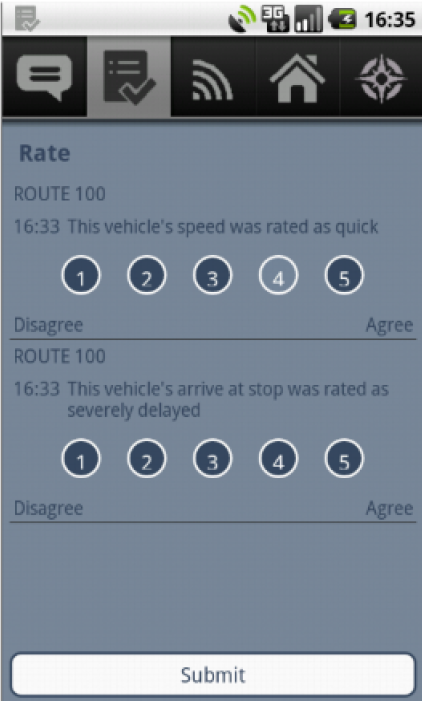
\includegraphics[scale=0.6]{rate_tab.png}
    \caption{Screenshot of the tab where we could find the rate comment feature.}
    \label{fig:iso}
  \end{center}
\end{figure}

\pagebreak

All these questions and conclusions led to the development of a initial interface redesign, presented in the following section.

\section{Initial Proposals}\label{sec:initial}

After the initial process of perceiving what was done before, as well as understanding what were the advantages and disadvantages of the previous design decisions, and what went well and could go better, there was a group of decisions to be made concerning what the next steps would be. Those decisions consisted of:

\begin{itemize}
\item Technology - Despite being still on a premature phase, what technology would be used in order to develop the functional prototype? In this case, since that prototype is expected to be an \emph{Android} application, what would be the versions targeted for the prototype?

\item Main Navigation - How to design the main navigation for the application? Stick by the use of the tabs? Explore other solutions used in similar contexts? 

\item Information shown on User Profile - What is relevant to be shown to the user? Does the user wants to see nearby users? Is he willing to allow his location to be shared and to see where are the users generating useful information to them? Or does he want to focus on more personal information, such as possible rewards, points, statistics and so on?

\item Comment, Rate and News Feed features - Can these be aggregated in a way user understands or is familiar with, or it represents an excessive amount of information to be shown in one screen? 

\item Journey Planner features - Could other features with perceived utility to the user be added in order to allow a better comprehension of the concept behind the application, and consequently, a more efficient use (for instance, saving time and avoiding repetitive tasks)?

\end{itemize}


\section{Focus Group}